% small.tex
\documentclass[10pt]{beamer}
\usetheme{default}

\usepackage{graphics}   % for pdf, bitmapped graphics files
\usepackage{epsfig}     % for postscript graphics files
\usepackage[font=footnotesize]{caption}

% Custom Commands
\newcommand{\sVec}[1]{\begin{bmatrix} #1 \end{bmatrix}}
\newcommand{\hl}[1]{ {\color{red} #1} }

% Variable definitions
\newcommand{\rot}{\boldsymbol\omega}
\newcommand{\trans}{\boldsymbol\nu}
\newcommand{\T}{\mathbf{T}}
\newcommand{\Tes}{\hat{\mathbf{T}}}
\newcommand{\twist}{\boldsymbol\xi}
\newcommand{\bu}{\mathbf{u}}
\newcommand{\bp}{\mathbf{p}}
\newcommand{\bn}{\mathbf{n}}
\newcommand{\bI}{\mathbf{I}}
\newcommand{\I}{\mathcal{I}}


\title{Monocular Visual Odometry}
%\subtitle{}
\author[C. Forster]{Christian Forster}
\institute[RPG]{
  Robotics and Perception Group \\
  Institute for Informatics \\
  University of Z\"urich
}
\date{December 9, 2013}
\begin{document}

\begin{frame}[plain]
  \titlepage
\end{frame}

\begin{frame}{Feature-based Visual Odometry}
	\begin{columns}
	  \begin{column}{0.4\textwidth}
	  	\begin{block}{Goal}
	  		\emph{Estimate relative pose $\T_{k,k-1}$ of new frame w.r.t. previous frame.}
	  	\end{block}
	  	\begin{block}{Pipeline}
		  	\begin{enumerate}
				\item Feature selection
				\item Feature matching 
				\item Pose estimation
				\item Pose refinement
				\item Triangulation
			\end{enumerate}
		\end{block}
	  \end{column}
	  \begin{column}{0.6\textwidth}
	    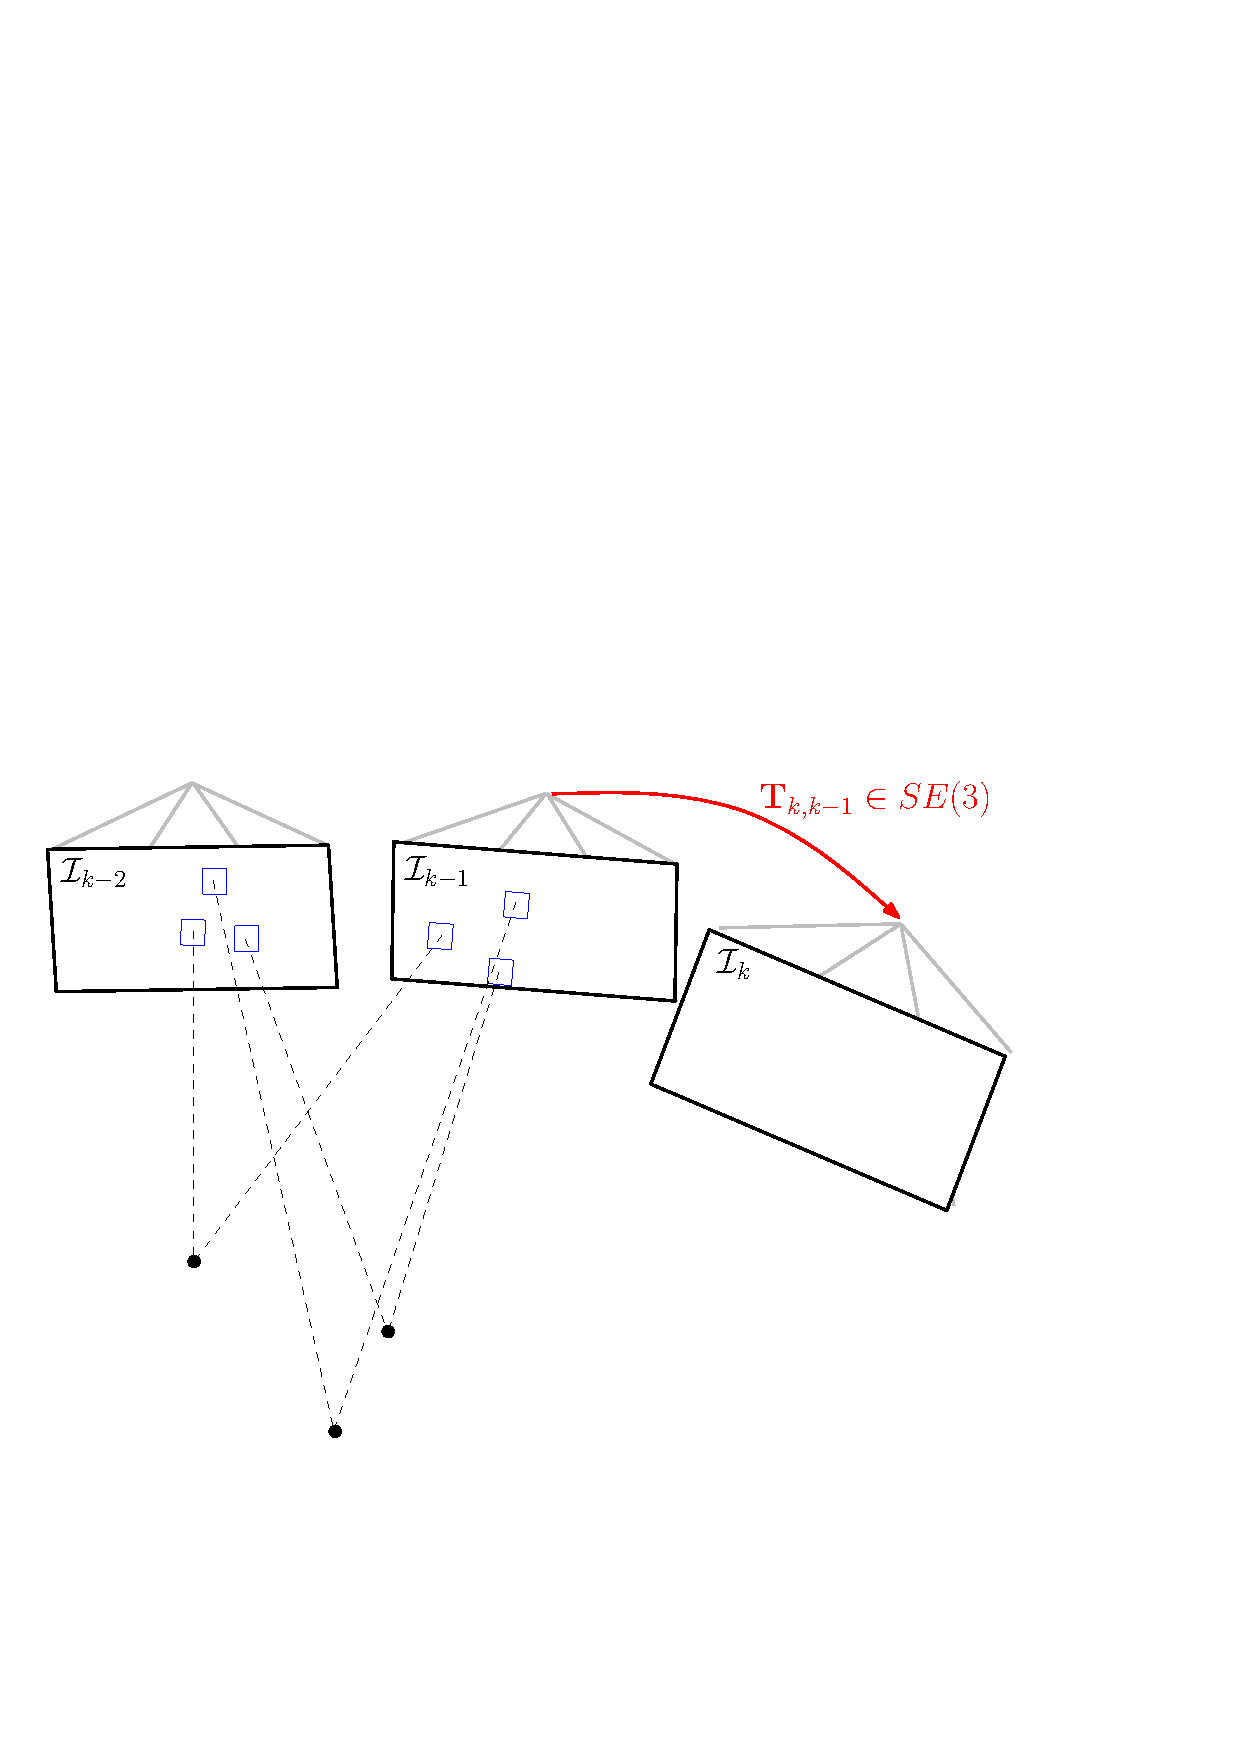
\includegraphics[width=\textwidth]{img/vo_pipeline_2}
	  \end{column}
	\end{columns}
\end{frame}

\begin{frame}{Feature-based Visual Odometry}
	\begin{columns}
	  \begin{column}{0.4\textwidth}
	  	\begin{block}{Pipeline}
		  	\begin{enumerate}
				\item \colorbox{yellow}{Feature selection}
				\item Feature matching 
				\item Pose estimation
				\item Pose refinement
				\item Triangulation
			\end{enumerate}
		\end{block}
		\begin{block}{Which features?}
			\vspace{0.3cm}
			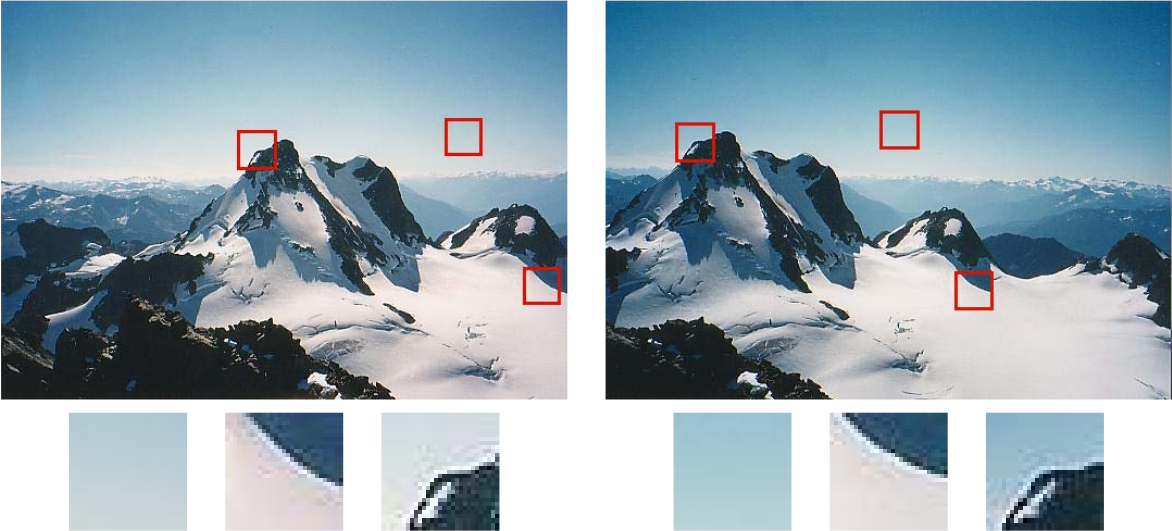
\includegraphics[width=\textwidth]{img/feature_selection.png}
			\vspace{0.1cm}
  			\tiny{\emph{Source: Szeliski, ``Computer Vision: Algorithms and Applications'', Springer 2010.}}
		\end{block}
	  \end{column}
	  \begin{column}{0.6\textwidth}
	    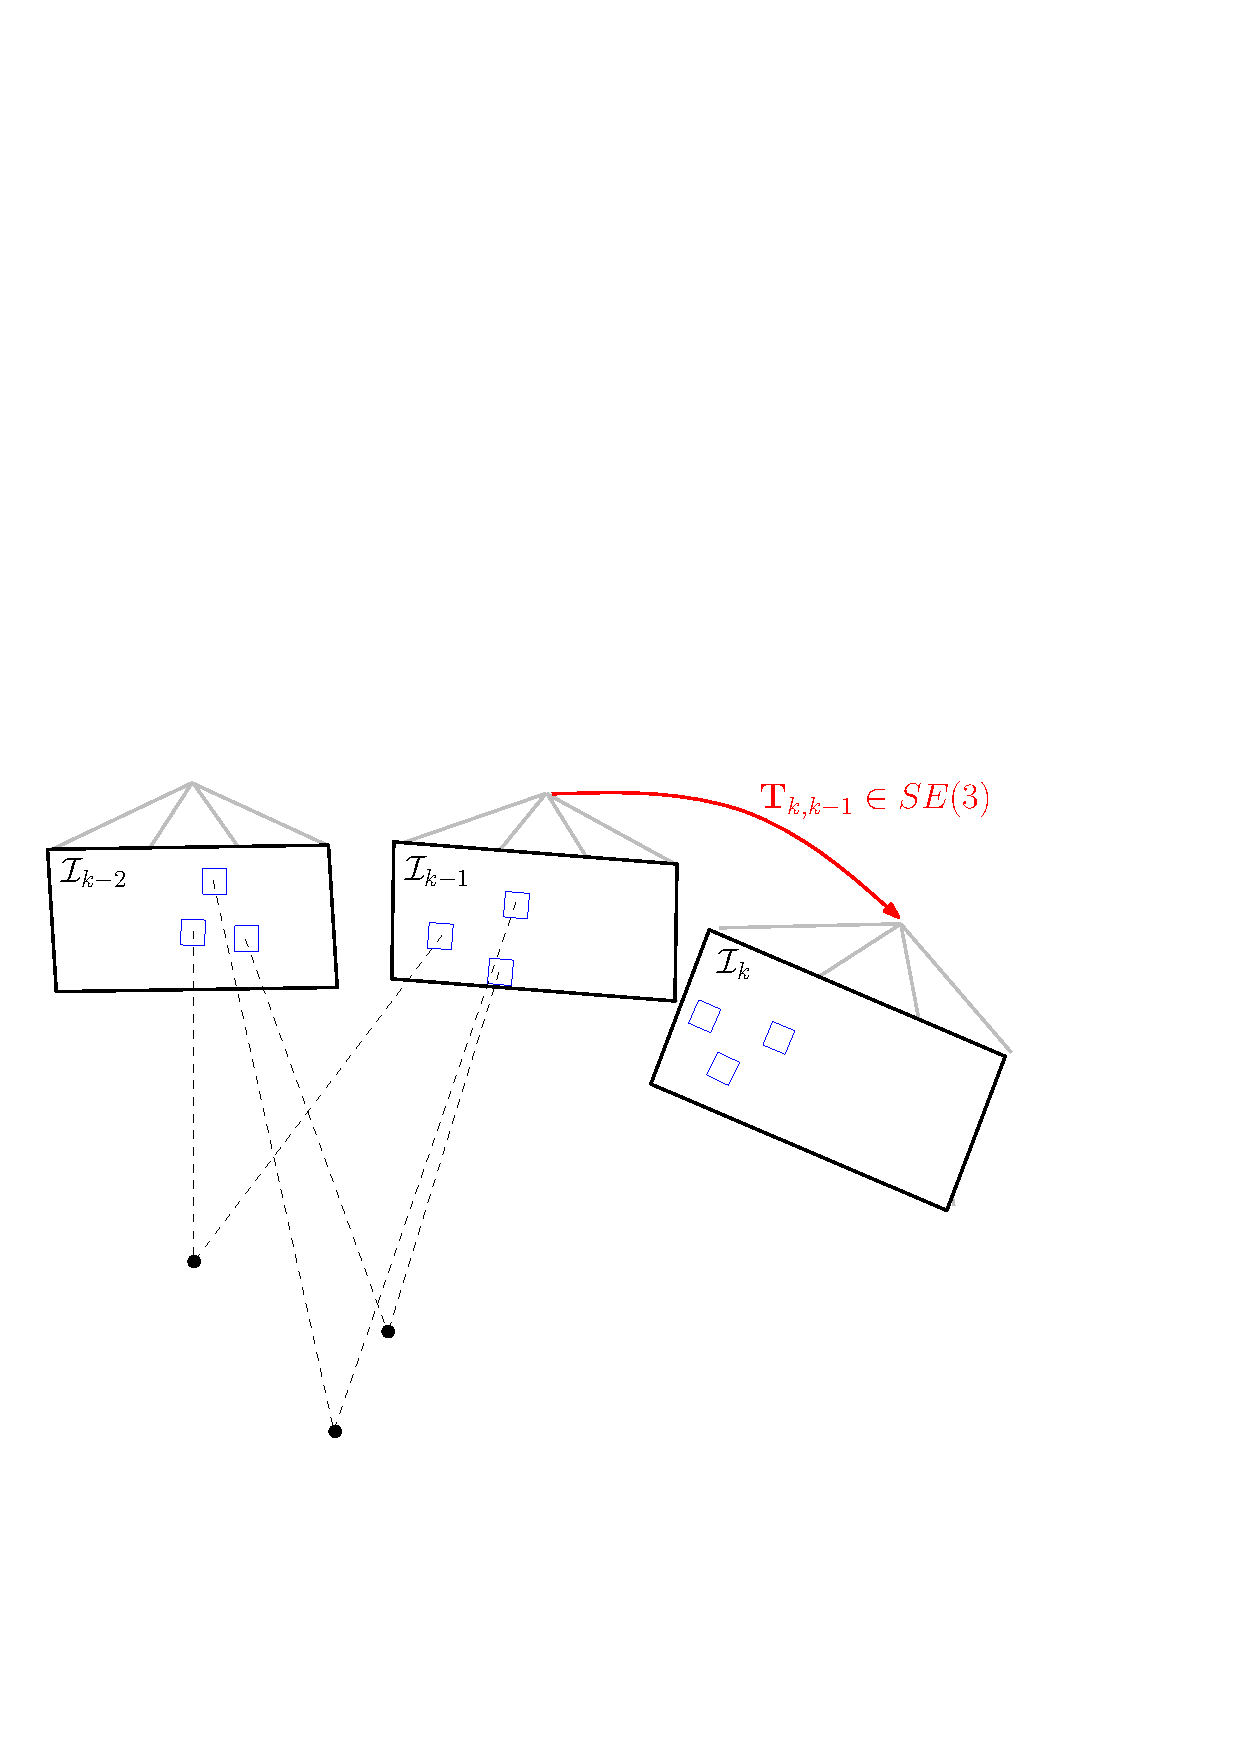
\includegraphics[width=\textwidth]{img/vo_pipeline_3}
	  \end{column}
	\end{columns}
\end{frame}

\begin{frame}{Feature-based Visual Odometry}
	\begin{columns}
	  \begin{column}{0.4\textwidth}
	  	\begin{block}{Pipeline}
		  	\begin{enumerate}
				\item Feature selection
				\item \colorbox{yellow}{Feature matching }
				\item Pose estimation
				\item Pose refinement
				\item Triangulation
			\end{enumerate}
		\end{block}
		\begin{block}{Matching Strategies}
			\begin{itemize}
				\item Fast: SSD/NCC over small patch
				\item Robust: Match invariant feature descriptors
			\end{itemize}
		\end{block}
	  \end{column}
	  \begin{column}{0.6\textwidth}
	    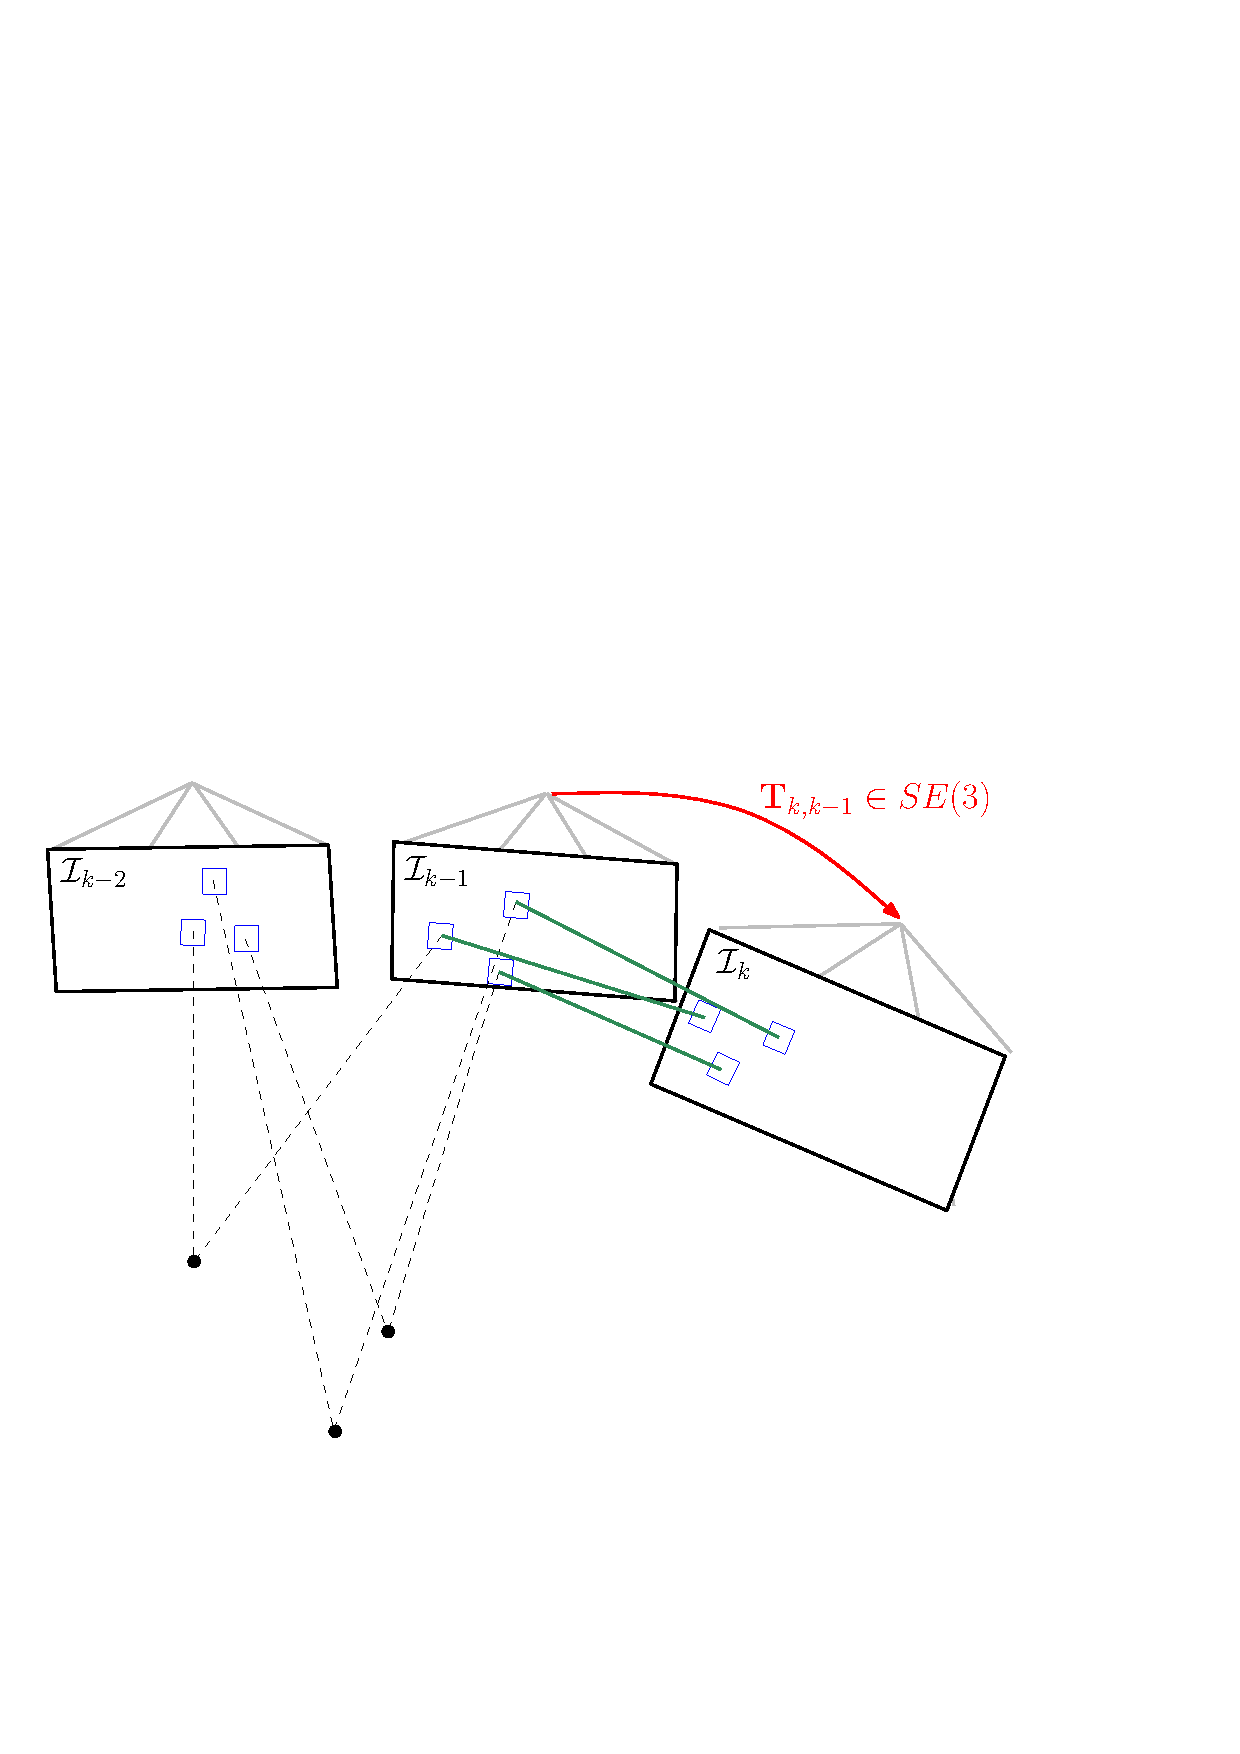
\includegraphics[width=\textwidth]{img/vo_pipeline_4}
	  \end{column}
	\end{columns}
\end{frame}

\begin{frame}{Feature-based Visual Odometry}
	\begin{columns}
	  \begin{column}{0.4\textwidth}
	  	\begin{block}{Pipeline}
		  	\begin{enumerate}
				\item Feature selection
				\item Feature matching
				\item \colorbox{yellow}{Pose estimation}
				\item Pose refinement
				\item Triangulation
			\end{enumerate}
		\end{block}
		\begin{block}{Epipolar Geometry}
			Three 3D point to 2D feature correspondences are necessary to estimate the 3D camera pose.
		\end{block}
	  \end{column}
	  \begin{column}{0.6\textwidth}
	    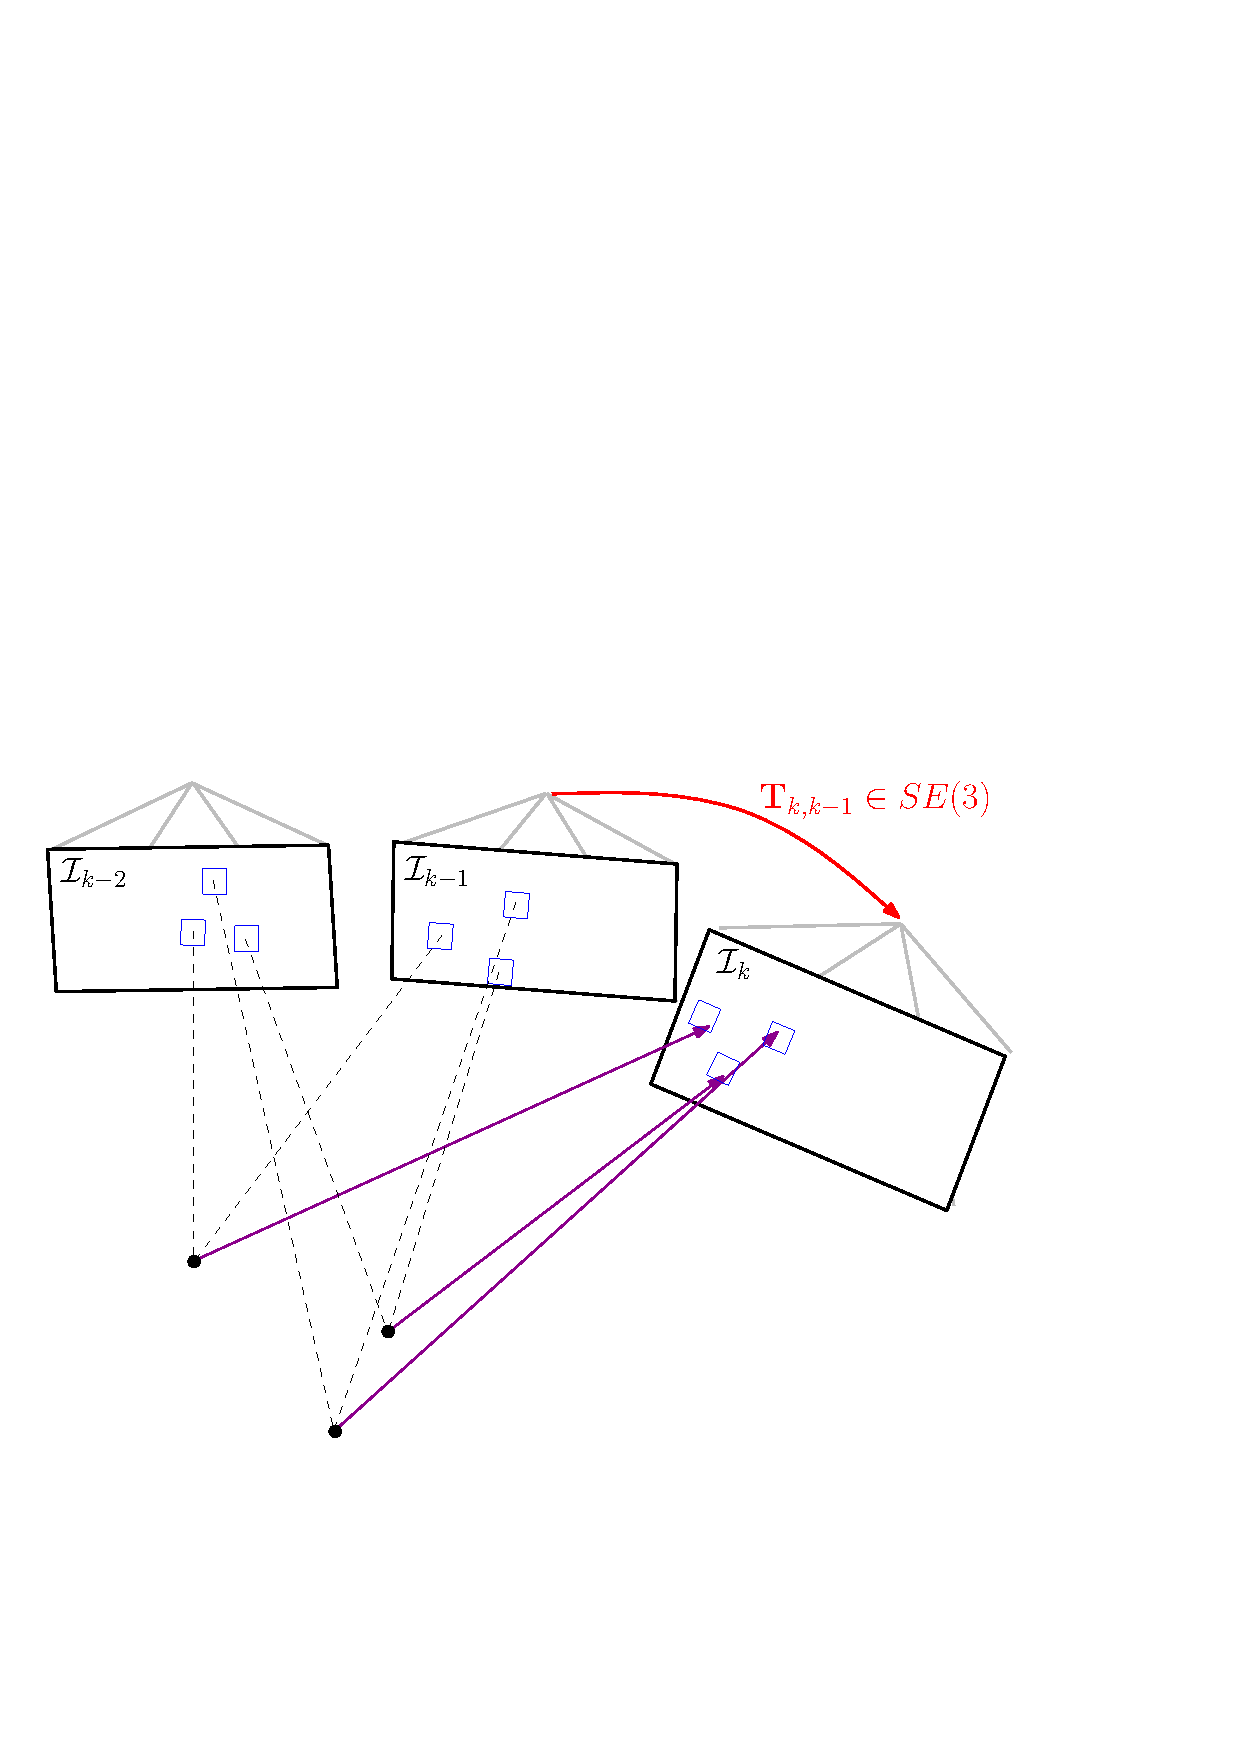
\includegraphics[width=\textwidth]{img/vo_pipeline_5}
	  \end{column}
	\end{columns}
\end{frame}

\begin{frame}{Feature-based Visual Odometry}
	\begin{columns}
	  \begin{column}{0.4\textwidth}
	  	\begin{block}{Pipeline}
		  	\begin{enumerate}
				\item Feature selection
				\item Feature matching
				\item Pose estimation
				\item \colorbox{yellow}{Pose refinement}
				\item Triangulation
			\end{enumerate}
		\end{block}
		\begin{block}{Minimize reprojection errors}
			\[
				\begin{aligned}
  				\T_{k,k-1} &= \\
  				       \arg&\min_{\T} \frac{1}{2} \sum_{i} \parallel \bu_i - \pi(\T \ _{k-1}\bp_i) \parallel^2.
  				\end{aligned}
			\]
			Can be solved with Gauss Newton.
		\end{block}
	  \end{column}
	  \begin{column}{0.6\textwidth}
	    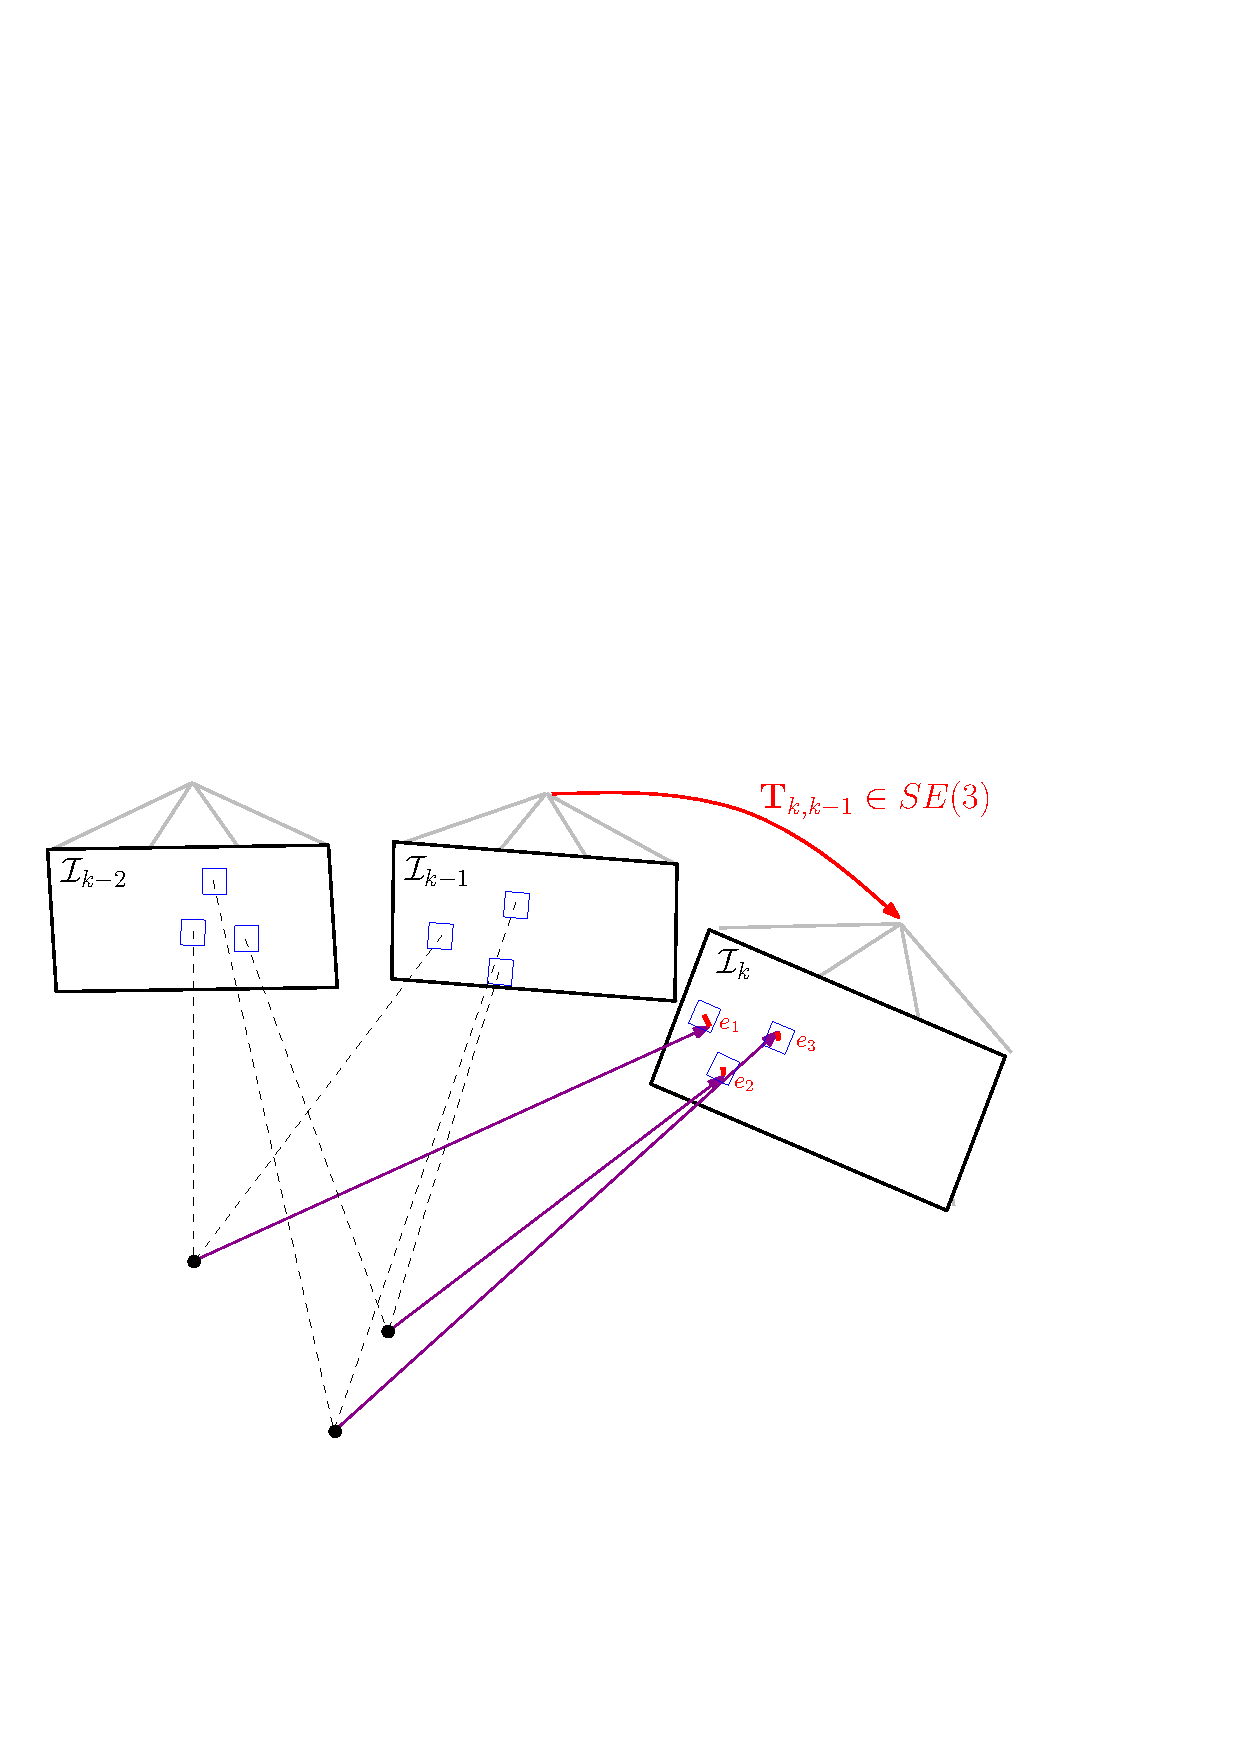
\includegraphics[width=\textwidth]{img/vo_pipeline_6}
	  \end{column}
	\end{columns}
\end{frame}

\begin{frame}{Feature-based Visual Odometry}
	\begin{columns}
	  \begin{column}{0.4\textwidth}
	  	\begin{block}{Pipeline}
		  	\begin{enumerate}
				\item Feature selection
				\item Feature matching
				\item Pose estimation
				\item Pose refinement
				\item \colorbox{yellow}{Triangulation}
			\end{enumerate}
		\end{block}
		\begin{block}{Triangulation}
			Search along Epipolar line for matching feature.
		\end{block}
	  \end{column}
	  \begin{column}{0.6\textwidth}
	    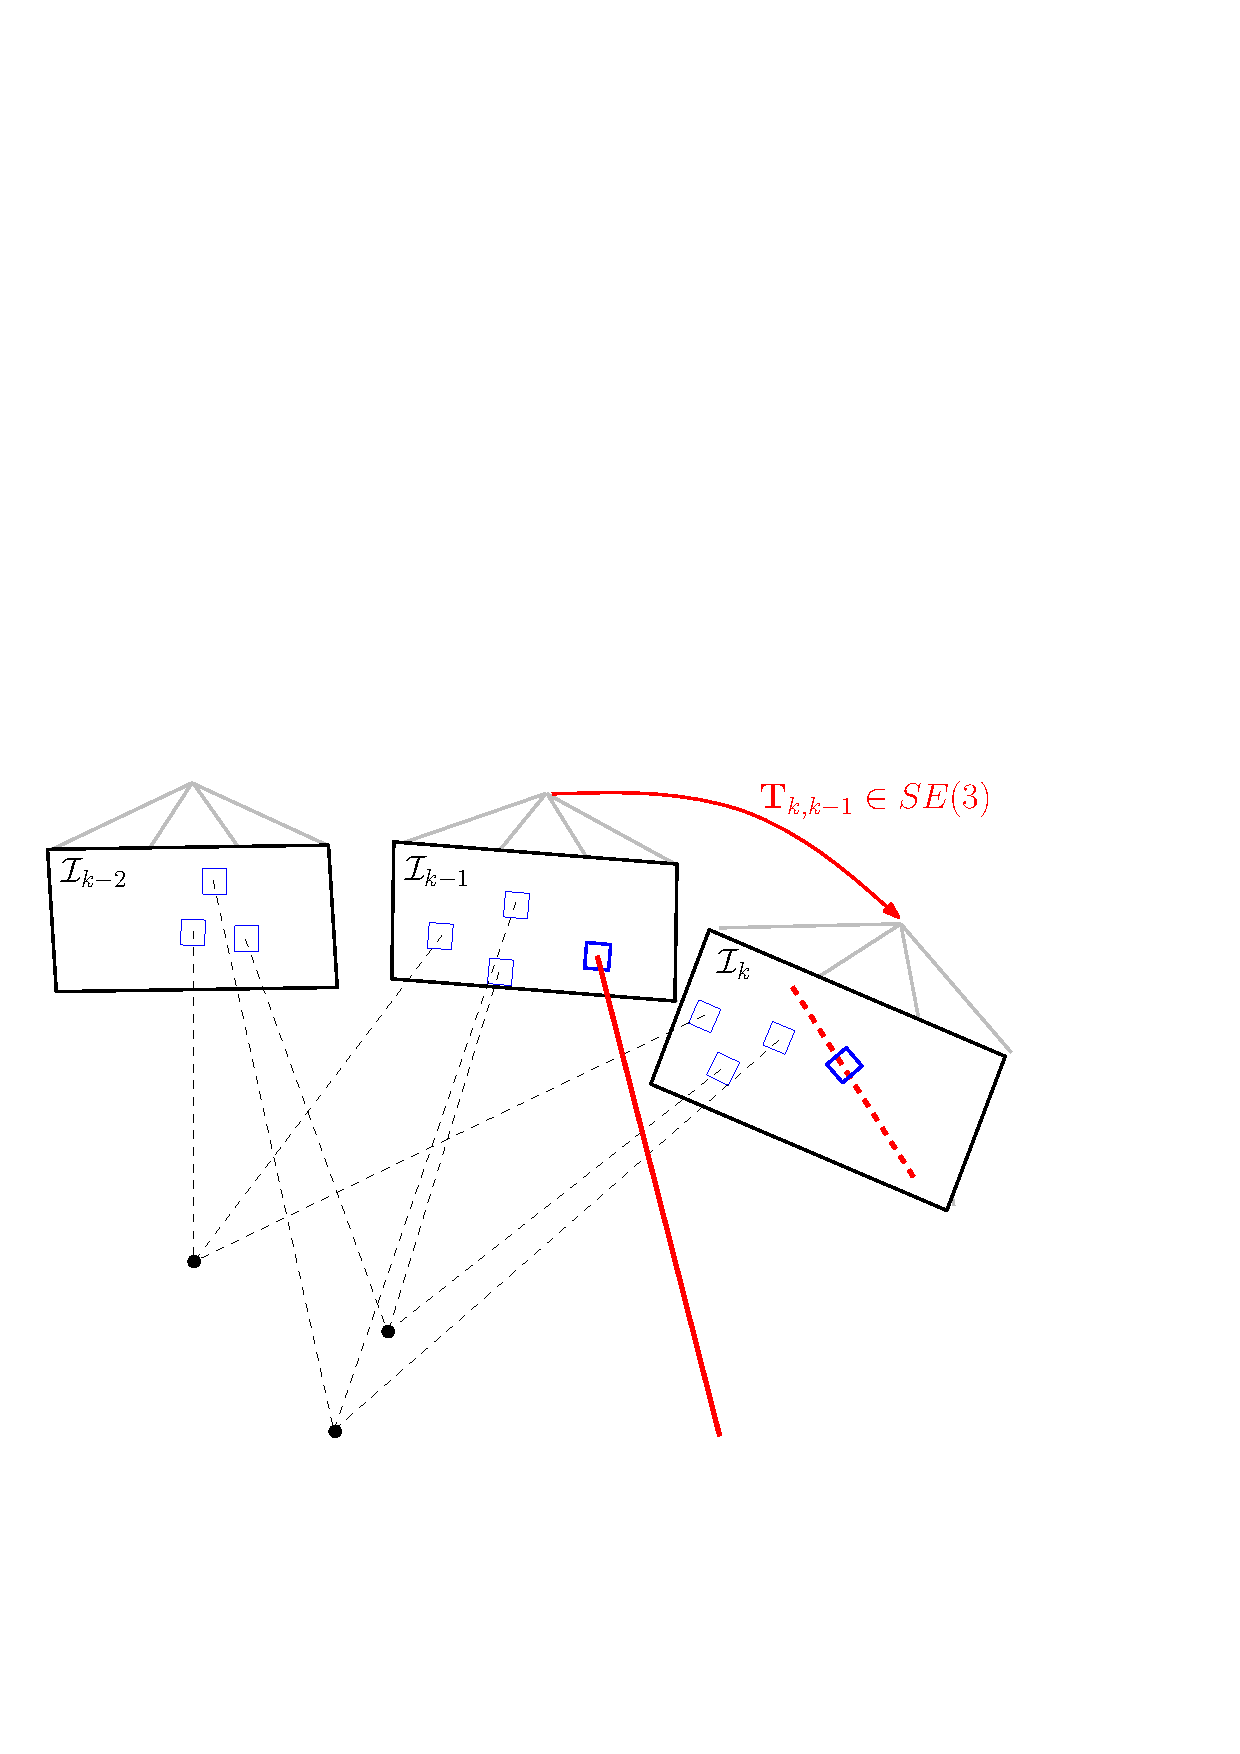
\includegraphics[width=\textwidth]{img/vo_pipeline_7}
	  \end{column}
	\end{columns}
\end{frame}

\begin{frame}{Feature-based Visual Odometry}
	\begin{columns}
	  \begin{column}{0.4\textwidth}
	  	\begin{block}{Pipeline}
		  	\begin{enumerate}
				\item Feature selection
				\item Feature matching
				\item Pose estimation
				\item Pose refinement
				\item \colorbox{yellow}{Triangulation}
			\end{enumerate}
		\end{block}
		\begin{block}{Triangulation}
			Search along Epipolar line for matching feature.
		\end{block}
	  \end{column}
	  \begin{column}{0.6\textwidth}
	    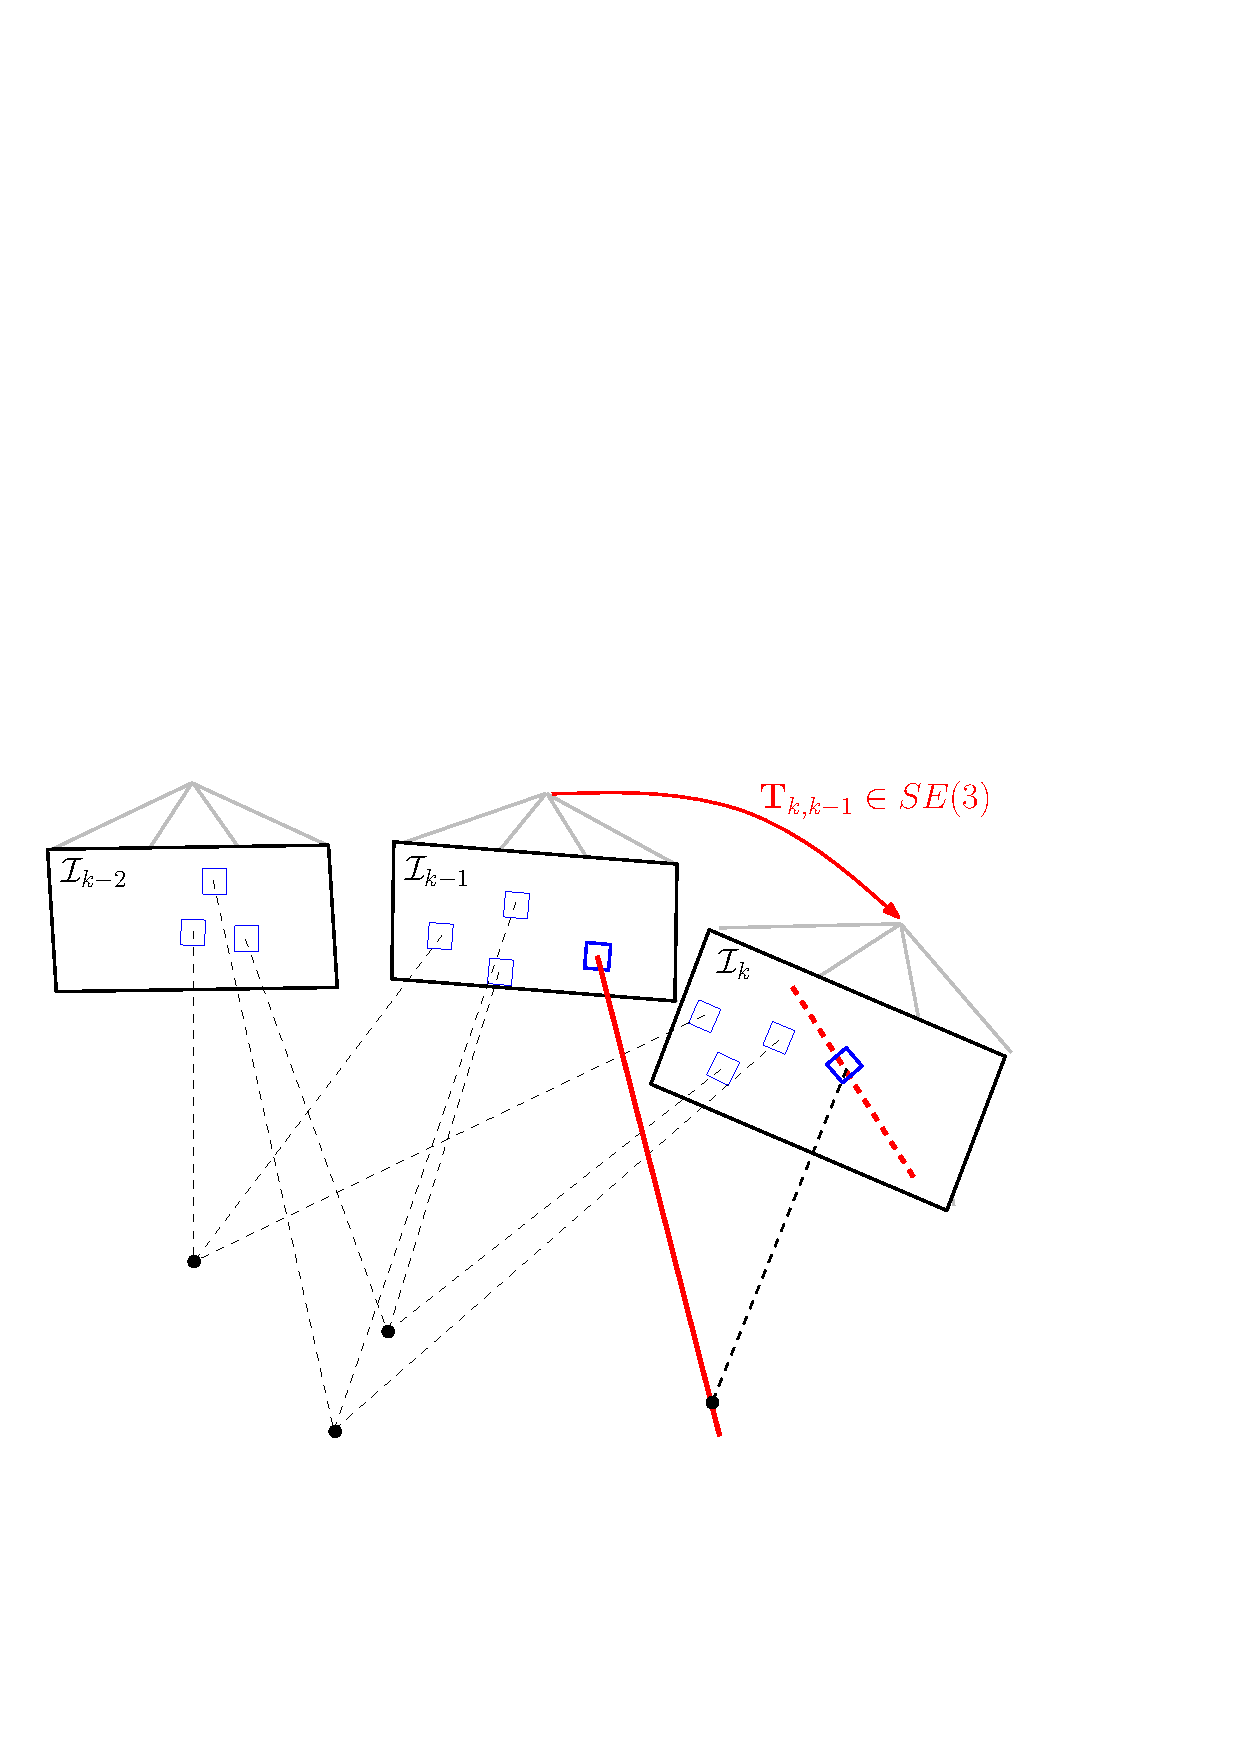
\includegraphics[width=\textwidth]{img/vo_pipeline_8}
	  \end{column}
	\end{columns}
\end{frame}

%----------- slide --------------------------------------------------%
\begin{frame}{Dense Tracking}
\[
  \T_{k,k-1} = \arg\min_\T \iint_{\bar{\mathcal{R}}} \rho\Big[ \delta \I\big(\T, \bu\big) \Big] d\bu.
\]
\[
  \delta \I\big(\T, \bu\big)
   = \I_k\Big(\pi\big(\T \cdot \pi^{-1}(\bu, z_\bu)\big)\Big) - \I_{k-1}(\bu) 
   \quad \forall \ \bu \in \bar{\mathcal{R}},
\]

\begin{itemize}
  \item itemized item 1
  \item itemized item 2
  \item itemized item 3
\end{itemize}

\begin{theorem}
  In a right triangle, the square of hypotenuse equals
  the sum of squares of two other sides.
\end{theorem}

\end{frame}

\end{document}